%!TEX root = /Users/louis/Documents/PhD/Deliverables/Thesis/thesis.tex

\section{Epsilon Flock: A Model Migration Language}
\label{sec:flock}
Driven by the analysis presented above, a domain-specific language for model migration, Epsilon Flock (subsequently referred to as Flock), has been designed and implemented. Flock makes idiomatic a novel and complicated semantics for automatically copying model elements from original to migrated model and a domain-specific language was preferred to repurposing an existing language to capture the semantics with a compact and tailored syntax. Section~\ref{subsec:flock_design} discusses the principle tenets of Flock, which include user-defined migration rules and a novel algorithm for relating source and target model elements. In Section~\ref{subsec:flock_examples}, Flock is demonstrated via application to three examples of model migration. Finally, Section~\ref{subsec:flock_guide} provides an overview of the ways in which a metamodel developer can use Flock to develop, test and distribute migration strategies. The work described in this section has been published in \cite{rose10flock}.

\subsection{Design and Implementation}
\label{subsec:flock_design}
Flock has been designed to be a rule-based transformation language that mixes declarative and imperative parts. Consequently, Flock should be familiar to developers who have used hybrid-style M2M transformation languages, such as ATL and ETL \cite{kolovos08etl}. Flock is syntactically efficient, but semantically complex. In particular, the way in which Flock relates source to target elements is novel; it is neither a new- nor an existing-target relationship. Instead, elements are copied conservatively, as described below.

Like Epsilon HUTN (Section~\ref{subsec:epsilon_hutn}), Flock reuses parts of Epsilon. In particular, Flock reuses EMC to provide interoperability with several modelling frameworks, and EOL for specifying the imperative part of user-defined migration rules.

\subsubsection{Abstract Syntax}
\label{subsubsec:abstract_syntax}
As illustrated by Figure~\ref{fig:abstract_syntax}, Flock migration strategies are organised into modules (\texttt{Fl\-ockMo\-du\-le}). Flock modules inherit from EOL modules (\texttt{Eo\-lMod\-ule}) and hence provide language constructs for specifying user-defined operations and for re-using modules. Flock modules comprise any number of rules (\texttt{Ru\-le}). Each rule has an original metamodel type (\texttt{or\-ig\-in\-alTy\-pe}) and can optionally specify a \texttt{gu\-ard}, which is either an EOL statement or a block of EOL statements. \texttt{Mi\-gr\-ateRu\-le}s must specify an evolved metamodel type (\texttt{ev\-ol\-vedTy\-pe}) and/or a \texttt{bo\-dy} comprising a block of EOL statements.

\begin{figure}[htb]
  \centering
  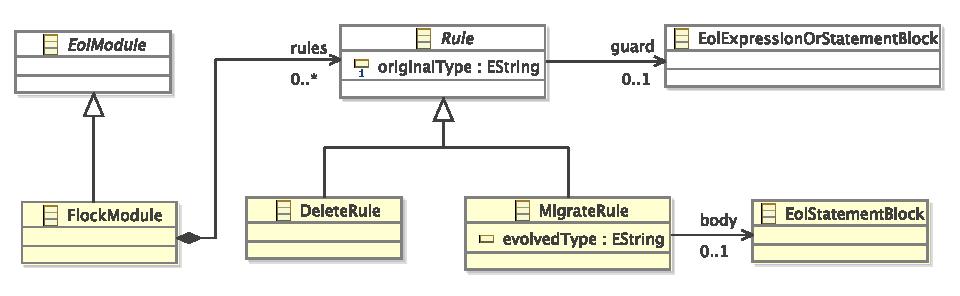
\includegraphics[scale=0.75]{5.Implementation/flock_abstract_syntax.pdf}
  \caption{The abstract syntax of Flock.}
  \label{fig:abstract_syntax}
\end{figure}

\subsubsection{Concrete Syntax}
\label{subsubsec:concrete_syntax}

Listing~\ref{lst:flock_concrete_syntax} shows the concrete syntax of migrate and delete rules. All rules begin with a keyword indicating their type (either \texttt{migrate} or \texttt{delete}), followed by the original metamodel type. Guards are specified using the \texttt{when} keywords. Migrate rules may also specify an evolved metamodel type using the \texttt{to} keyword and a \texttt{body} as a (possibly empty) sequence of EOL statements.

Note that Flock does not define a create rule. The creation of new model elements is instead encoded in the imperative part of a migrate rule specified on the containing type.

\begin{lstlisting}[float=tbp, caption=Concrete syntax of migrate and delete rules., label=lst:flock_concrete_syntax, language=Flock]
migrate <originalType> (to <evolvedType>)?
(when (:<eolExpression>)|({<eolStatement>+}))? {
	<eolStatement>*
} 

delete <originalType>
(when (:<eolExpression>)|({<eolStatement>+}))?
\end{lstlisting}

\subsubsection{Execution Semantics}
\label{subsubsec:execution_semantics}
When executed, a Flock module consumes an original model, \texttt{O}, and constructs a migrated model, \texttt{M}. The transformation is performed in three phases: rule selection, equivalence establishment and rule execution. The behaviour of each phase is described below, and the first example in Section~\ref{subsec:flock_examples} demonstrates the way in which a Flock module is executed.

\paragraph{Rule Selection}
The rule selection phase determines an \emph{applicable} rule for every model element, \texttt{e}, in \texttt{O}. As such, the result of the rule selection phase is a set of pairs of the form \texttt{<r,e>} where \texttt{r} is a migration rule.

A rule, \texttt{r}, is \emph{applicable} for a model element, \texttt{e}, when the original type of \texttt{r} is the same type as (or is a supertype of) the type of \texttt{e}; and the guard part of \texttt{r} is satisfied by \texttt{e}.

The rule selection phase has the following behaviour:

\begin{itemize}
	\item For each original model element, \texttt{e}, in \texttt{O}:
	\subitem $-$ Identify for \texttt{e} the set of all applicable rules, \texttt{R}. Order \texttt{R} by the occurrence of rules in the Flock source file.
	\subsubitem $\circ$ If \texttt{R} is empty, let \texttt{r} be a default rule, which has the type of \texttt{e} as both its original and evolved type, and an empty body.
	\subsubitem $\circ$ Otherwise, let \texttt{r} be the first element of \texttt{R}.
	\subitem $-$ Add the pair \texttt{<r,e>} to the set of selected rules.
\end{itemize}

Rules are ordered according to their position in the Flock source file. A rule that appears earlier (higher) in the source file has priority. Ordering rules according to generality is an alternative approach for distinguishing between applicable rules \cite{wallace05modular}. In model transformation, the generality of a rule might be assessed by considering its source type and guard. For Flock, the former approach was preferred, because it simplified implementation and is consistent with the way in which rules are selected in other languages of the Epsilon platform.

\paragraph{Equivalence Establishment}
The equivalence establishment phase creates an equivalent model element, \texttt{e'}, in M for every pair of rules and original model elements, \texttt{<r,e>}. The equivalence establishment phase produces a set of triples of the form \texttt{<r,e,e'>}, and has the following behaviour:

\begin{itemize}
	\item For each pair \texttt{<r,e>} produced by the rule selection phase:
	\subitem $-$ If \texttt{r} is a delete rule, do nothing.
	\subitem $-$ If \texttt{r} is a migrate rule:
	\subsubitem $\circ$ Create a model element, \texttt{e'}, in M. The type of \texttt{e'} is determined from the the \texttt{evolvedType} (or the \texttt{originalType} when no \texttt{evolvedType} has been specified) of \texttt{r}.
	\subsubitem $\circ$ Copy the data contained in \texttt{e} to \texttt{e'} (using the \emph{conservative copy} algorithm described in the sequel).
	\subsubitem $\circ$ Add the triple \texttt{<r,e,e'>} to the set of equivalences.
\end{itemize}
	
\paragraph{Rule Execution}
The final phase executes the imperative part of the user-defined migration rules on the set of triples \texttt{<r,e,e'>}, and has the following behaviour:

\begin{itemize}
	\item For each triple \texttt{<r,e,e'>} produced by the equivalence establishment phase:
	\subitem $-$ Bind \texttt{e} and \texttt{e'} to new EOL variables named \texttt{or\-ig\-in\-al} and \texttt{mi\-gr\-at\-ed}, respectively.
	\subitem $-$ Execute the body of \texttt{r} with EOL.
\end{itemize}


\subsubsection{Conservative Copy}
\label{subsubsec:conservative_copying}
Flock contributes a novel algorithm, termed \emph{conservative copy}, that copies model elements from original to migrated model only when those model elements conform to the evolved metamodel. Conservative copy is a hybrid of the new- and existing-target source-target relationships that are commonly used in M2M transformation \cite{czarnecki06survey}, because some model elements are copied from source to target (as in an existing-target transformation), while some model elements must be copied explicitly (as in a new-target transformation).

Conservative copy operates on an original model element, \texttt{e}, and its equivalent model element in the migrated model, \texttt{e'}, and has the following behaviour:

\begin{itemize}
	\item For each metafeature, \texttt{f} for which \texttt{e} has specified a value:
		\subitem $-$ Find a metafeature, \texttt{f'}, of \texttt{e'} with the same name as \texttt{f}.
			\subsubitem $\circ$ If no equivalent metafeature can be found, do nothing.
			\subsubitem $\circ$ Otherwise, copy the original value (\texttt{e.f}) to produce a migrated value (\texttt{e'.f'}) if and only if the migrated value conforms to \texttt{f'}.
\end{itemize}

The definition of conformance varies over modelling frameworks. Typically, conformance between a value, \texttt{v}, and a feature, \texttt{f}, specifies at least the following constraints:

\begin{itemize}
	\item The size of \texttt{v} must be greater than or equal to the lowerbound of \texttt{f}.
	\item The size of \texttt{v} must be less than or equal to the upperbound of \texttt{f}.
	\item The type of \texttt{v} must be the same as or a subtype of the type of \texttt{f}.
\end{itemize}

EMC provides drivers for several modelling frameworks, permitting management of models defined with EMF, the Metadata Repository (MDR), Z or XML. To support migration between metamodels defined in heterogeneous modelling frameworks, EMC has been extended to support conformance checking; each EMC driver provides conformance checking semantics specific to its modelling framework. Specifically, EMC define Java interfaces for specifying the way in which model values are written to a model, and an additional, conformance checking Java method has been added to the interface. When a Flock module is executed, conformance checking responsibilities are delegated to EMC drivers by calling the new method. The conformance checking support in EMC is applicable to other areas of the Epsilon platform and, in particular, could be used to add some static type checking to the Epsilon languages, which are currently dynamically typed.

In response to some types of metamodel evolution, some categories of model value must be converted before being copied from the original to the migrated model. Again, the need for and semantics of this conversion varies over modelling frameworks. For example, reference values typically require conversion before copying because, once copied, they must refer to elements of the migrated rather than the original model. In this case, the set of equivalences (\texttt{<r,e,e'>}) can be used to perform the conversion. In other cases, the target modelling framework must be used to perform the conversion, such as when EMF enumeration literals are copied.

% \subsubsection{Partial Migration}
% Existing co-evolution tools consume and produce conformant models (Section~\ref{sec:subsec:modelling_framework_characteristics}), and hence tools cannot typically be combined to decompose model migration. By re-using the metamodel-independent syntax (Section~\ref{sec:mmi_syntax}), Flock can consume and produce non-conformant models, and hence can be used in combination with other co-evolution tools that support non-conformant models.
% 
% To integrate Flock with the metamodel-independent syntax, an additional driver was added to EMC. The additional driver allows a model to be loaded, manipulated and stored in a manner that is not constrained by the structures and rules defined by its metamodel. Epsilon HUTN (Section~\ref{subsec:epsilon_hutn}) and Flock can be used together to perform migration, because both are interoperable with the metamodel-independent syntax. For example, migration can be performed by executing a Flock migration strategy to automatically produce a partially migrated (non-conformant) model. Subsequently, Epsilon HUTN can then be used to manually reconcile any remaining non-conformant model elements to produce a migrated (conformant) model. Decomposing model migration facilitates collaborative and incremental co-evolution.

\subsection{Examples of Flock Migration}
\label{subsec:flock_examples}
Flock is now demonstrated using three examples of model migration. The first example demonstrates the way in which a Flock module is executed and illustrates the semantics of conservative copy. The second describes the way in which the migration of the Petri net co-evolution example (Section~\ref{subsec:co-evo_example}) can be specified with Flock, and is included for direct comparison with the other languages discussed in Section~\ref{sec:analyis_of_languages_used_for_migration}. The final, larger example demonstrates all of the features of Flock, and is based on changes made to UML class diagrams between versions 1.5 and 2.0 of the UML specification.

\subsubsection{Process-Oriented Migration in Flock}
The first example considers the evolution of a process-oriented metamodel, introduced in \ref{sec:other_examples} and described in . The process-oriented metamodel was developed to explore the feasibility of a graphical model editor for representing programs written in process-oriented programming languages, such as occam-$\pi$ \cite{occam_pi}.

\begin{figure}[htb]
	\centering
	\subfigure[Original metamodel.]
	{
	    \label{fig:cc_eg_original}
	    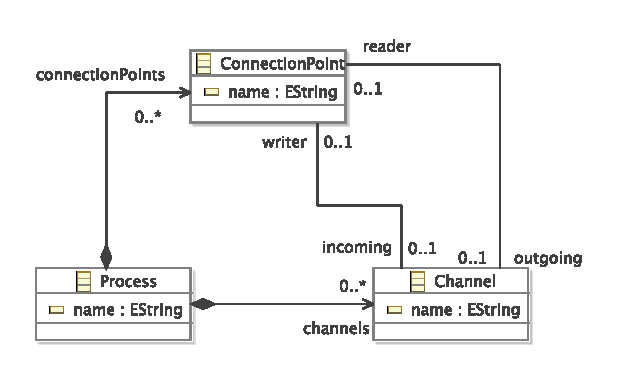
\includegraphics[width=8.5cm]{5.Implementation/images/cc_eg_original.pdf}
	}
	\subfigure[Evolved metamodel.]
	{
	    \label{fig:cc_eg_evolved}
	    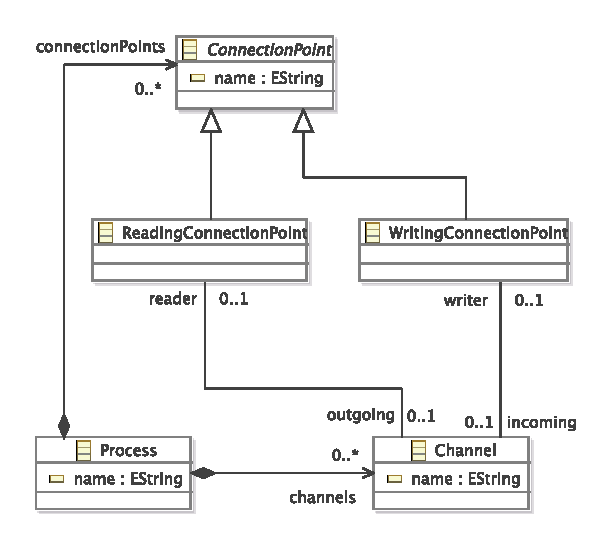
\includegraphics[width=8.5cm]{5.Implementation/images/cc_eg_evolved.pdf}
	}
	\caption[Evolution of the Process-Oriented metamodel]{Evolution of the Process-Oriented metamodel (Appendix~\ref{ProcessOriented})}
\label{fig:cc_eg_mms}
\end{figure}

The original metamodel, shown in Figure~\ref{fig:cc_eg_original}, has been evolved to distinguish between \texttt{Co\-nn\-ec\-ti\-o\-nP\-oi\-nt}s that are a reader for a \texttt{Ch\-an\-n\-el} and \texttt{Co\-nn\-ec\-ti\-o\-nP\-oi\-nt}s that are a writer for a \texttt{Ch\-an\-n\-el} by making \texttt{Co\-nn\-ec\-ti\-o\-nP\-oi\-nt} abstract and introducing two subtypes, \texttt{Re\-a\-di\-ngCo\-nn\-ec\-ti\-o\-nP\-oi\-nt} and \texttt{Wr\-i\-ti\-ngCo\-nn\-ec\-ti\-o\-nP\-oi\-nt}, as shown in Figure~\ref{fig:cc_eg_evolved}.

The model shown in Figure~\ref{fig:cc_eg_model} conforms to the original metamodel in Figure~\ref{fig:cc_eg_original} and is to be migrated. The model comprises three \texttt{Pr\-oc\-e\-ss}es named \emph{delta}, \emph{prefix} and \emph{minus}; three \texttt{Ch\-an\-n\-el}s named \emph{a}, \emph{b} and \emph{c}; and six \texttt{Co\-nn\-ec\-ti\-o\-nP\-oi\-nt}s named \emph{a?}, \emph{a!}, \emph{b?}, \emph{b!}, \emph{c?} and \emph{c!}.

\begin{figure}[htbp]
	\centering
		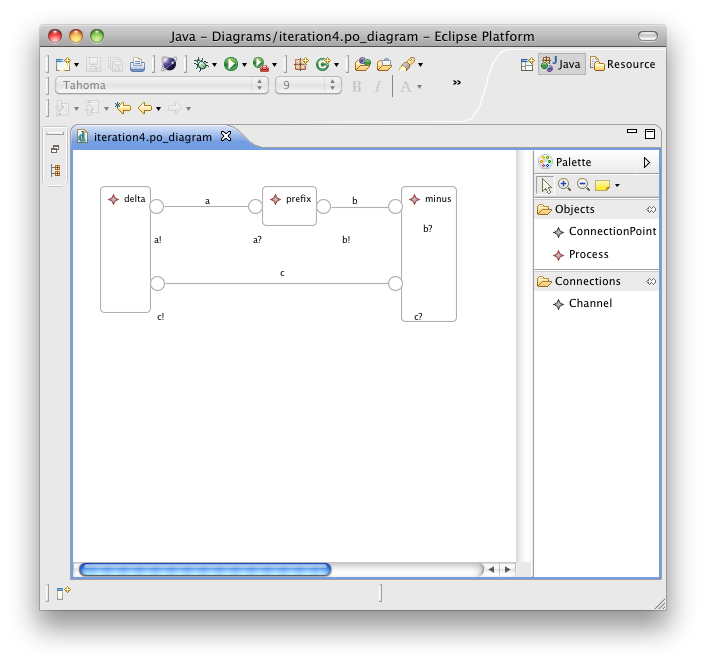
\includegraphics[scale=0.5]{A.2.ProcessOriented/images/4_model.png}
	\caption{Process-Oriented model prior to migration}
	\label{fig:cc_eg_model}
\end{figure}

\begin{lstlisting}[float=tbp, caption=Redefining equivalences for the Component model migration., label=lst:cc_eg_rules, language=Flock]
migrate ConnectionPoint to ReadingConnectionPoint when: original.outgoing.isDefined()
migrate ConnectionPoint to WritingConnectionPoint when: original.incoming.isDefined()
\end{lstlisting}

For the migration strategy shown in Listing~\ref{lst:cc_eg_rules}, the Flock module will perform the following steps. Firstly, the rule selection phase produces a set of pairs \texttt{<r,e>}. For each \texttt{ConnectionPoint}, the guard part of the user-defined rules control which rule will be selected. \texttt{ConnectionPoint}s \texttt{a!}, \texttt{b!} and \texttt{c!} have outgoing \texttt{Channel}s (\texttt{a}, \texttt{b} and \texttt{c} respectively) and hence the migration rule on line 1 is selected. Similarly, the \texttt{ConnectionPoint}s \texttt{a?}, \texttt{b?} and \texttt{c?} have incoming \texttt{Channel}s (\texttt{a}, \texttt{b} and \texttt{c} respectively) and hence the migration rule on line 2 is selected. There is no \texttt{ConnectionPoint} with both an outgoing and an incoming \texttt{Channel}, but if there were, the first applicable rule (i.e. the rule on line 1) would be selected. For the other model elements (the \texttt{Process}es and \texttt{Channel}s) no user-defined rules are applicable, and so default rules are used instead. A default rule has an empty body and identical original and evolved types. In other words, a default rule for the \texttt{Process} type is equivalent to the user-defined rule: \texttt{migrate Process to Process \{\}}

Secondly, the equivalence establishment phase creates an element, \texttt{e'}, in the migrated model for each pair \texttt{<r,e>}. For each \texttt{ConnectionPoint}, the evolved type of the selected rule (\texttt{r}) controls the type of \texttt{e'}. The rule on line 1 of Listing~\ref{lst:cc_eg_rules} was selected for the \texttt{ConnectionPoint}s \texttt{a!}, \texttt{b!} and \texttt{c!} and hence an equivalent element of type \texttt{ReadingConnectionPoint} is created for \texttt{a!}, \texttt{b!} and \texttt{c!}. Similarly, an equivalent element of type \texttt{WritingConnectionPoint} is created for \texttt{a?}, \texttt{b?} and \texttt{c?}. For the other model elements (the \texttt{Process}es and \texttt{Channel}s) a default rule was selected, and hence the equivalent model element has the same type as the original model element.

Finally, the rule execution phase performs a conservative copy for each original and equivalent model element in the set of triples \texttt{<r,e,e'>} produced by the equivalence establishment phase. The metamodel evolution shown in Figure~\ref{fig:cc_eg_mms} has not affected the \texttt{Pr\-oc\-e\-ss} type, and hence for each \texttt{Pr\-oc\-e\-ss} in the original model, conservative copy will create a \texttt{Pr\-oc\-e\-ss} in the migrated model and copy the values of all features. For each \texttt{Ch\-an\-n\-el} in the original model, conservative copy will create an equivalent \texttt{Ch\-an\-n\-el} in the migrated model and copy the value of the \texttt{na\-me} feature from original to migrated model element. However, the values of the \texttt{re\-ad\-er} and \texttt{wr\-it\-er} features will not be copied by conservative copy because the type of these features has changed (from \texttt{Co\-nn\-ec\-ti\-o\-nP\-oi\-nt} to \texttt{Re\-a\-di\-ngCo\-nn\-ec\-ti\-o\-nP\-oi\-nt} and \texttt{Wr\-i\-ti\-ngCo\-nn\-ec\-ti\-o\-nP\-oi\-nt}, respectively). The values of the \texttt{re\-ad\-er} and \texttt{wr\-it\-er} features in the original model will not conform to the \texttt{re\-ad\-er} and \texttt{wr\-it\-er} features in the evolved metamodel. Finally, the values of the \texttt{na\-me}, \texttt{in\-co\-mi\-ng} and \texttt{ou\-tg\-oi\-ng} features of the \texttt{Co\-nn\-ec\-ti\-o\-nP\-oi\-nt} class have not evolved, and hence are copied directly from original to equivalent model elements.

The rule execution phase also executes the body of each rule, \texttt{r}, for every triple in the set \texttt{<r,e,e'>}. The user-defined rules in Listing~\ref{lst:cc_eg_rules} have no body, and hence no further execution is performed in this case.

\subsubsection{Petri Nets Migration in Flock}
The Petri net metamodel evolution demonstrates the core functionality of Flock. In Listing~\ref{lst:flock}, \texttt{Net}s and \texttt{Place}s are migrated automatically. Unlike the ATL migration strategy (Listing~\ref{lst:atl}), no explicit copying rules are required. Compared to the COPE migration strategy (Listing~\ref{lst:cope}), the Flock migration strategy does not need to unset the original \texttt{src} and \texttt{dst} features of \texttt{Transition}.

\begin{lstlisting}[caption=Petri nets model migration in Flock, label=lst:flock, language=Flock]
migrate Transition {
  for (source in original.src) {
    var arc := new Migrated!PTArc;
    arc.src := source.equivalent();  arc.dst := migrated;
    arc.net := original.net.equivalent();
  }

  for (destination in original.dst) {
    var arc := new Migrated!TPArc;
    arc.src := migrated;  arc.dst := destination.equivalent();
    arc.net := original.net.equivalent();
  }
}
\end{lstlisting}

\subsubsection{UML Class Diagram Migration in Flock}
Figure~\ref{fig:uml_mms} illustrates a subset of the changes made between UML 1.5 and UML 2.0. Only class diagrams are considered, and features that did not change are omitted. In Figure~\ref{fig:original_uml_mm}, association ends and attributes are specified separately. In Figure~\ref{fig:evolved_uml_mm}, the \texttt{Pr\-op\-er\-ty} class is used instead. The Flock migration strategy (Listing~\ref{lst:flock-uml}) for Figure~\ref{fig:uml_mms} is now discussed.

Firstly, \texttt{At\-tr\-ib\-ut\-e}s and \texttt{As\-so\-ci\-at\-i\-onEn\-d}s are migrated to be \texttt{Pr\-o\-pe\-rt\-ies} (lines 14 to 18, and 25 to 29). In particular, the \texttt{As\-so\-ci\-at\-i\-on\#na\-vi\-ga\-b\-leEn\-ds} reference replaces the \texttt{As\-so\-ci\-at\-i\-onE\-nd\#isN\-av\-ig\-ab\-le} attribute; following migration, each navigable \texttt{As\-so\-ci\-at\-i\-onE\-nd} must be referenced via the \texttt{na\-vi\-ga\-bl\-eEn\-ds} feature of its \texttt{As\-so\-ci\-at\-ion} (lines 26-28).

In UML 2.0, \texttt{St\-ru\-ct\-ur\-alFe\-at\-ur\-e\#o\-wn\-er\-Sc\-op\-e} has been replaced by \texttt{\#i\-sS\-ta\-ti\-c} (lines 15-17 and 20-22). The UML 2.0 specification states that the UML 1.5 values \texttt{Sc\-op\-eKi\-nd\#cl\-as\-si\-fi\-er} and \texttt{\#i\-ns\-ta\-nce} should be migrated to true and to false, respectively. 

The UML 1.5 \texttt{St\-ru\-ct\-ur\-alFe\-at\-ur\-e\#t\-ar\-g\-et\-Sc\-op\-e} feature is no longer supported in UML 2.0, and no migration path is provided. Consequently, line 14 deletes any model element whose \texttt{t\-ar\-g\-et\-Sc\-op\-e} is not the default value.

Finally, \texttt{C\-la\-ss\#fe\-at\-ur\-es} has been split to form \texttt{C\-la\-ss\#op\-er\-at\-io\-ns} and \texttt{\#at\-tr\-ib\-ut\-es}. Lines 7 and 8 partition features on the original \texttt{Cl\-a\-ss} into \texttt{Op\-er\-at\-io\-n}s and \texttt{Pr\-op\-er\-ty}s. \texttt{Cl\-as\-s\#a\-ss\-oc\-ia\-ti\-on\-s} has been removed in UML 2.0, and \texttt{As\-so\-ci\-at\-i\-onEn\-d}s are instead stored in \texttt{Cl\-a\-ss\#at\-tr\-ib\-ut\-es} (line 9).

\begin{lstlisting}[caption=UML model migration in Flock, label=lst:flock-uml, language=Flock, float=tb]
migrate Association {
	migrated.memberEnds := original.connections.equivalent();
}

migrate Class {
	var fs := original.features.equivalent();
	migrated.operations := fs.select(f|f.isKindOf(Operation));
	migrated.attributes := fs.select(f|f.isKindOf(Property));
	migrated.attributes.addAll(original.associations.equivalent())
}

delete StructuralFeature when: original.targetScope <> #instance

migrate Attribute to Property {
	if (original.ownerScope = #classifier) {
		migrated.isStatic = true;		
	}
}
migrate Operation {
	if (original.ownerScope = #classifier) {
		migrated.isStatic = true;
	}
}

migrate AssociationEnd to Property {
	if (original.isNavigable) {
		original.association.equivalent().navigableEnds.add(migrated)
	}
}
\end{lstlisting}

\begin{landscape}	
\begin{figure}[ht]
	\centering
	\subfigure[Original, UML 1.5 metamodel.]
	{
	    \label{fig:original_uml_mm}
	    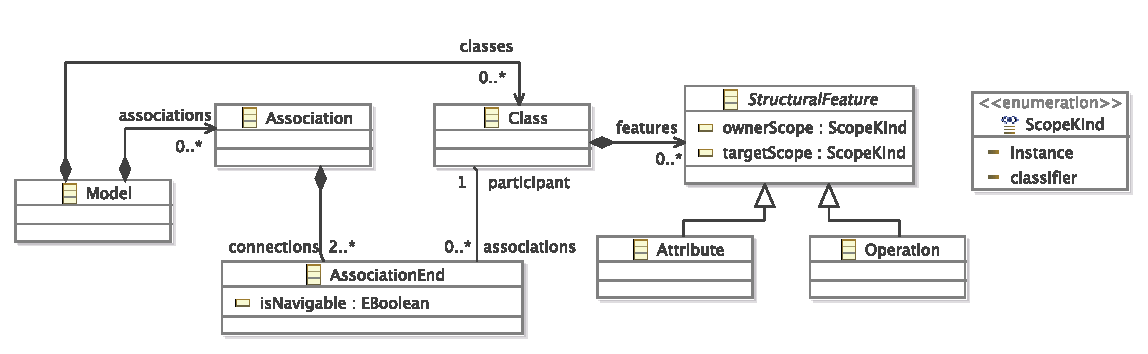
\includegraphics[width=15cm]{5.Implementation/images/uml_class_before.pdf}
	}
	\subfigure[Evolved, UML 2.0 metamodel.]
	{
	    \label{fig:evolved_uml_mm}
	    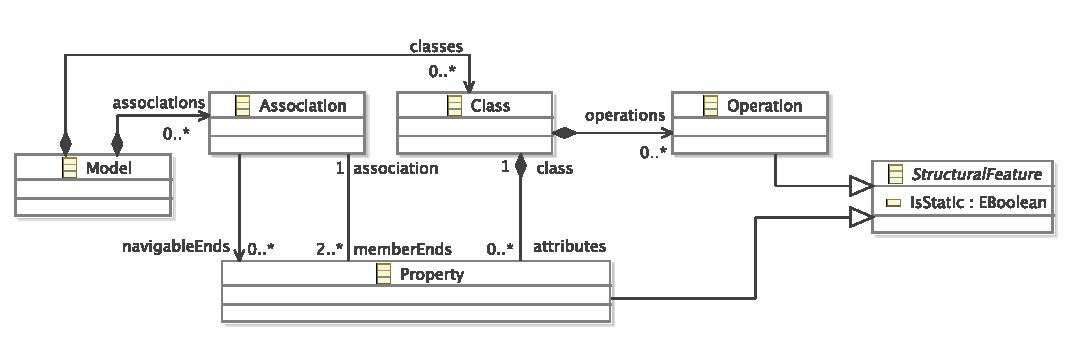
\includegraphics[width=15cm]{5.Implementation/images/uml_class_after.pdf}
	}
	\caption{UML metamodel evolution}
\label{fig:uml_mms}
\end{figure}
\end{landscape}	


\subsection{Developing Migration Strategies with Epsilon Flock}
\label{subsec:flock_guide}
The design and implementation of Flock and example migration strategies were presented in Sections~\ref{subsec:flock_design} and \ref{subsec:flock_examples} respectively. This section summarises the way in which Flock is integrated with Epsilon and Eclipse, and in particular discusses using Flock's development tools to construct and distribute migration strategies. Further information on developing migration strategies with Epsilon Flock can be found on the documentation section of Epsilon website\footnote{\url{http://www.eclipse.org/gmt/epsilon/doc/}} and, in particular, in the Epsilon book\footnote{\url{http://www.eclipse.org/gmt/epsilon/doc/book/}}.

\paragraph{Installation} Flock is distributed as part of Epsilon, and hence can installed via the Eclipse update manager, using the Epsilon update site. Detailed and up-to-date installation instructions are available from the Epsilon website\footnote{\url{http://www.eclipse.org/gmt/epsilon/download/}}. Once installed, Epsilon provides additional views, editors and wizards for specifying and executing model management operations, such as model migration with Flock.

\paragraph{Creating and editing migration strategies} New Flock migration strategies can be created from the \emph{File $>$ New File $>$ Other\ldots} menu by selecting \emph{Epsilon $>$ Epsilon Flock Migration Strategy}, as shown in Figure~\ref{fig:flock_new_migration_strategy}. The resulting file will be automatically opened with the Flock editor, which provides syntax highlighting and automatic error detection. In addition, the Flock editor is integrated with the Eclipse outline view, shown in the right-hand side of Figure~\ref{fig:flock_editor_and_outline_view}, which can be used to navigate between rules and operations in the current migration strategy.

\begin{figure}[tbp]
	\centering
		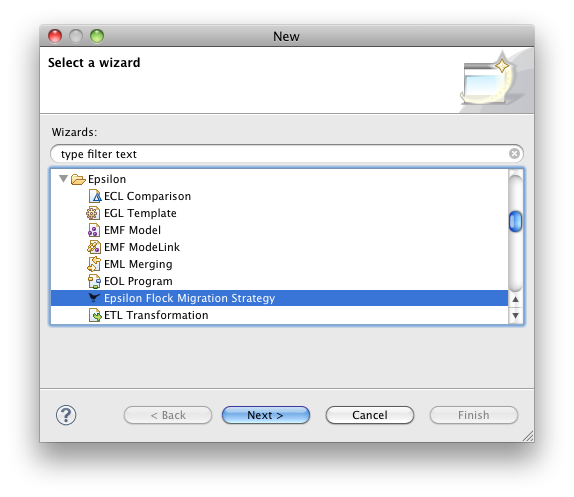
\includegraphics[height=9cm]{5.Implementation/images/flock_programmers_guide/new_migration_strategy.png}
	\caption{Creating a new migration strategy with Flock.}
	\label{fig:flock_new_migration_strategy}
\end{figure}


\begin{figure}[tbp]
	\centering
		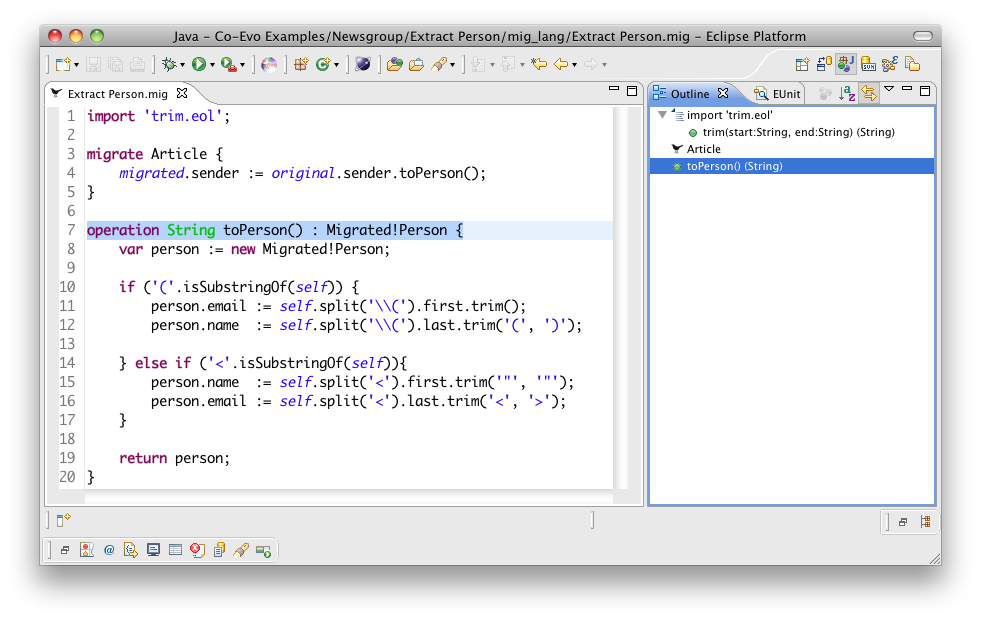
\includegraphics[height=8.5cm]{5.Implementation/images/flock_programmers_guide/editor.png}
	\caption{The Flock editor (left) and outline view (right).}
	\label{fig:flock_editor_and_outline_view}
\end{figure}


\paragraph{Executing migration strategies} Flock migration strategies can be executed from the \emph{Run $>$ Run Configurations\ldots} menu item, by selecting the Flock Migration Strategy category and clicking New, as shown in Figure~\ref{fig:flock_new_launch_config}. Next, the location of the Flock migration strategy and original and migrated models must be specified. The \emph{Source} tab (Figure~\ref{fig:flock_new_launch_config_source}) is used to specify the location of the Flock migration strategy to be executed, via the  \emph{Browse Workspace\ldots} button. The \emph{Models} tab (Figure~\ref{fig:flock_new_launch_config_models}) is used to specify the location of the original and evolved models. First, the add buttons are used to configure each model's properties, specifying, for example, an identifier, the location of the model and the location of its metamodel. Once the models' properties have been configured, drop down boxes are used to specify the role (\emph{Original} or \emph{Migrated}) of each model, as shown at the bottom of   Figure~\ref{fig:flock_new_launch_config_models}. After the locations of the migration strategy and models have been specified, the migration strategy is executed by clicking the \emph{Run} button.

More than two models can be specified when executing a Flock migration strategy. Although only one model can play the role of \emph{Original} or \emph{Migrated} model, extra models can be used to guide migration. For example, a migration strategy might query a third model to determine whether or not a migrate rule should be executed. More generally, an inference co-evolution approach (Section~\ref{subsec:inference}) could be implemented with Flock by using migration strategies in conjunction with a model of the metamodel differences. 

During the execution of a migration strategy, Flock constructs a migrated model in the location specified in the launch configuration (described above). The migrated model can be opened with the editors provided by the modelling framework. For example, an EMF model can be opened with a model editor generated by EMF, or with Epsilon's Exeed editor\footnote{\url{http://www.eclipse.org/gmt/epsilon/doc/exeed/}}; and an XML model can be opened with Eclipse's XML editor. Runtime errors are displayed in the Eclipse error log view, and textual output (e.g. the result of evaluating \texttt{pr\-in\-t\-ln()} statements) in the Eclipse console view.

\begin{figure}[tbp]
	\centering
		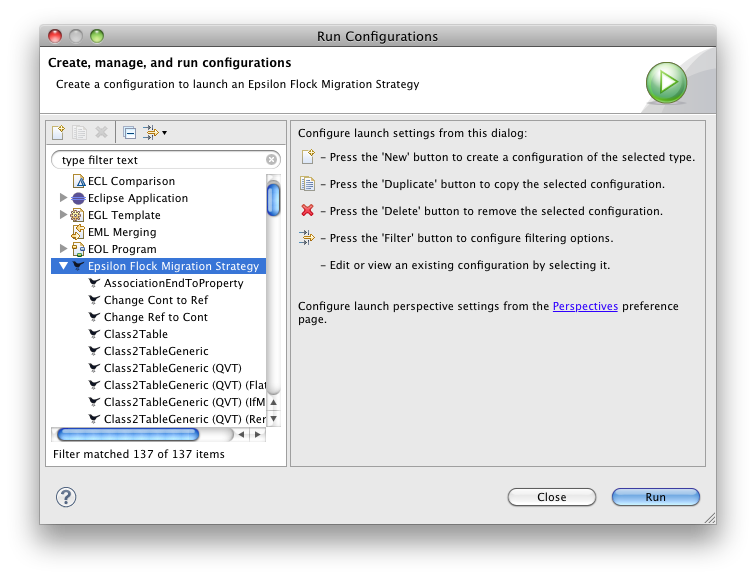
\includegraphics[height=8.5cm]{5.Implementation/images/flock_programmers_guide/new_launch_config.png}
	\caption{Creating a new run configuration for a Flock migration strategy.}
	\label{fig:flock_new_launch_config}
\end{figure}

\begin{figure}[tbp]
	\centering
		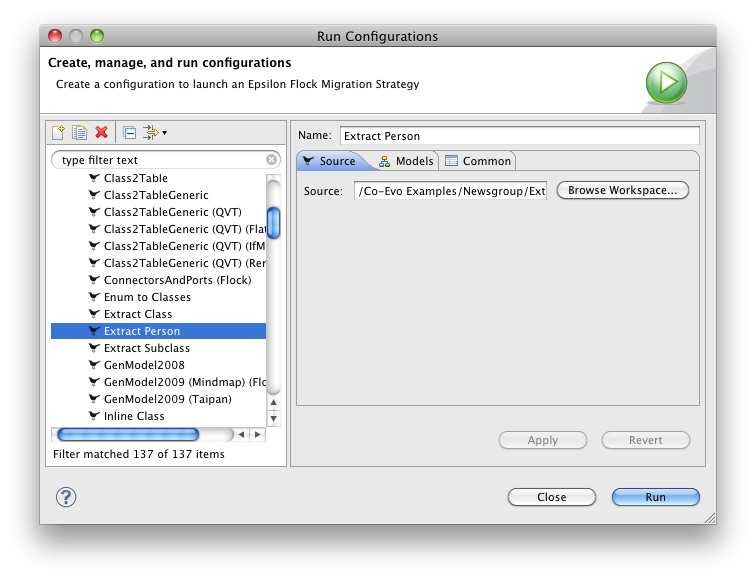
\includegraphics[height=8.5cm]{5.Implementation/images/flock_programmers_guide/new_launch_config_source.png}
	\caption{Configuring the source file for a Flock run configuration.}
	\label{fig:flock_new_launch_config_source}
\end{figure}

\begin{figure}[tbp]
	\centering
		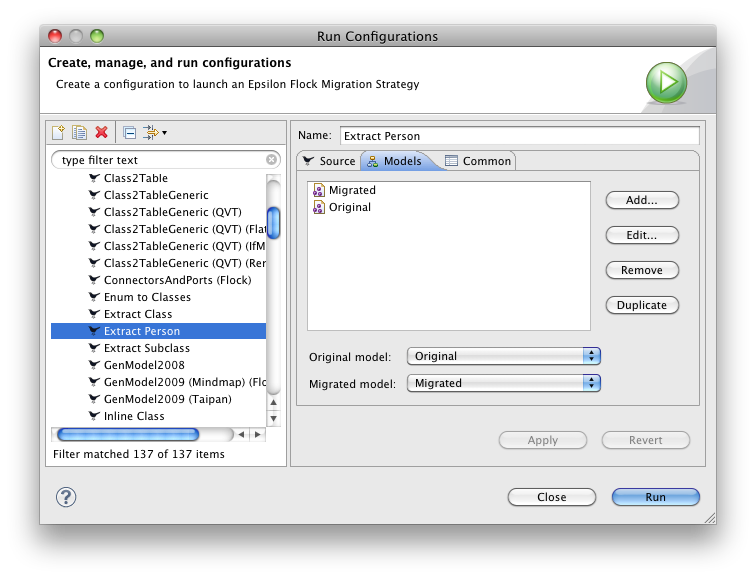
\includegraphics[height=8.5cm]{5.Implementation/images/flock_programmers_guide/new_launch_config_models.png}
	\caption{Configuring models for a Flock run configuration.}
	\label{fig:flock_new_launch_config_models}
\end{figure}

\paragraph{Distributing migration strategies} Metamodels and models are typically kept separate (Section~\ref{subsec:modelling_framework_characteristics}). EMF metamodels, for example, are typically packaged in Eclipse plug-ins and distributed to metamodel users. To facilitate the distribution of migration strategies to metamodel users, Flock provides a mechanism for including Flock migration strategies as part of an EMF metamodel plug-in. More specifically, Flock defines an Eclipse \emph{extension point}. To distribute a migration strategy to metamodel users, the metamodel developer creates an \emph{extension} (an instance of the Flock extension point) and specifies the location of the Flock migration strategy, the original metamodel and the evolved metamodel, as show in Figure~\ref{fig:flock_extension}. When metamodel users install a plug-in that contains a Flock extension, Flock provides a menu that can be used to invoke migration strategies, as shown in Figure~\ref{fig:flock_extension_execution}. Note that the metamodel developer can provide a file extension (when specifying the Flock extension) for which the \emph{Flock} menu will be displayed.

\begin{figure}[tbp]
	\centering
		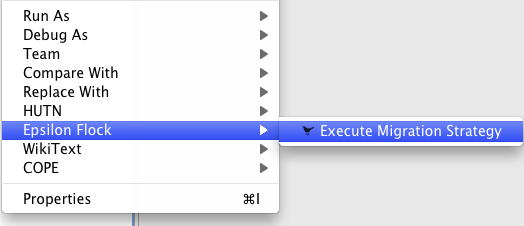
\includegraphics[height=4cm]{5.Implementation/images/flock_programmers_guide/extension_execution.png}
	\caption{Executing a migration strategy from a metamodel plug-in.}
	\label{fig:flock_extension_execution}
\end{figure}

Metamodel developers can also elect to build their own interface for invoking migration strategies, and delegate responsibility for executing migration strategies to the Flock execution engine. To this end, the \texttt{FlockModule} class (Section~\ref{subsec:flock_design}) provides a fa\c{c}ade \cite[pg185]{gamma95patterns} for the Flock execution engine, and an example use is shown in Listing~\ref{lst:flock_module_usage}. This approach to distributing migration strategies requires more effort from the metamodel developer (who must integrate the code in Listing~\ref{lst:flock_module_usage} with the development tools of the metamodel user), but is more flexible (and could be used, for example, to integrate model migration with model or source code management repositories).

\begin{landscape}
\begin{figure}[tbp]
	\centering
		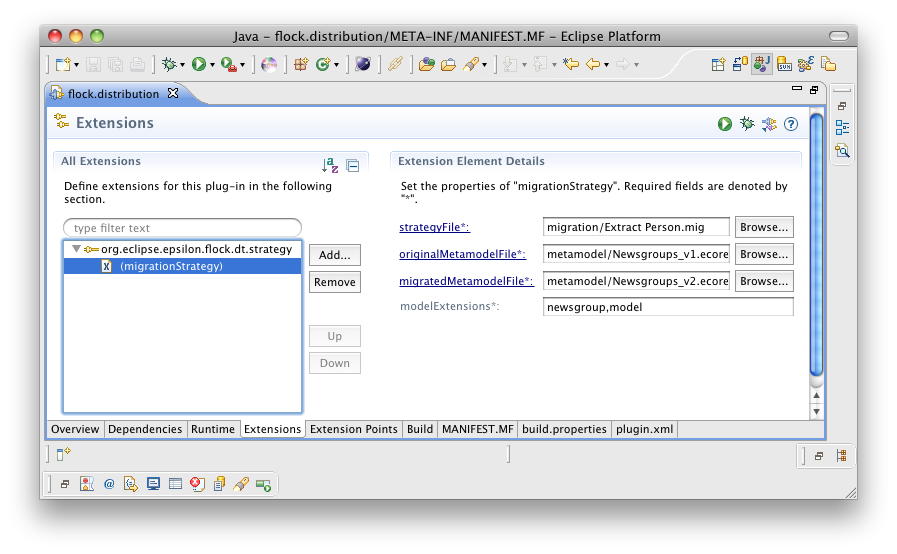
\includegraphics[height=11.5cm]{5.Implementation/images/flock_programmers_guide/extension.png}
	\caption{Distributing a migration strategy as part of a metamodel plug-in via a Flock extension.}
	\label{fig:flock_extension}
\end{figure}
\end{landscape}

\begin{lstlisting}[caption=Executing a Flock migration strategy programmatically in Java., label=lst:flock_module_usage, language=Java, float=tb]
private static void migrate(File strategy,
	                                   File originalModelFile,
                                     File migratedModelFile)
  throws Exception {
	
	final IFlockModule migrator = new FlockModule();
	
	final EmfModelFactory factory = EmfModelFactory.getInstance()
	final IModel original = factory.loadEmfModel("Original", originalModelFile, "originalMetamodelUri");
	final IModel migrated = factory.loadEmfModel("Original", migratedModelFile, "evolvedMetamodelUri");
	
	if (migrator.parse(strategy) &&
	     migrator.getParseProblems().isEmpty()) {		
		
		final FlockResult result = migrator.execute(original, migrated);
	
		result.printWarnings(System.err);
		
	} else {
		for (ParseProblem problem : migrator.getParseProblems()) {
			System.err.println(problem);
		}
	}
}
\end{lstlisting}

% \paragraph{Partial migration} Flock includes an additional model driver for EMC that facilitates the management of non-conformant models (Section~\ref{subsec:flock_design}). Therefore, Flock migration strategies can consume or produce non-conformant models. 

\subsection{Summary}
Requirements for a language tailored to model migration were described in Section~\ref{sec:analyis_of_languages_used_for_migration}. This section has presented Epsilon Flock, a language that seeks to fulfil those requirements. The way in which Flock has been designed and implemented has been discussed, with a particular focus on the novel source-target relationship, conservative copy (Section~\ref{subsec:flock_design}). Several examples of migration strategies constructed in Flock have been presented (Section~\ref{subsec:flock_examples}). Further examples are given in Appendix~\ref{CoevolutionExamples}. Finally, the way in which metamodel developers can use the Flock development tools to construct and distribute migration strategies was discussed (Section~\ref{subsec:flock_guide}).

Table~\ref{tab:differences} illustrates several characterising differences between Flock and the pre-existing languages presented in Section~\ref{sec:analyis_of_languages_used_for_migration}. Due to its conservative copying algorithm, Flock is the only language to provide both automatic copying and unsetting. The evaluation presented in Section~\ref{sec:quantitive} explores the extent to which automatic copying and unsetting affect the conciseness of migration strategies.

All of the approaches considered in Section~\ref{sec:analyis_of_languages_used_for_migration} support EMF. Both Flock and ATL support further modelling technologies, such as MDR and XML. However, ATL does not automatically copy model elements that have not been affected by metamodel changes. Therefore, migration between models of different technologies with ATL requires extra statements in the migration strategy to ensure that the conformance constraints of the target technology are satisfied. Because it delegates conformance checking to an EMC driver, Flock requires no such checks.

\begin{table}[tbp]
	\centering
	\begin{tabular}{|c|c|c|c|}
		\hline
		             & \multicolumn{2}{c|}{\textbf{Automatic}} & \textbf{Modelling} \\
		\textbf{Tool}& \textbf{Copy} & \textbf{Unset}          & \textbf{technologies} \\
		\hline
		Ecore2Ecore  & \tick             & \cross              & XMI                    \\
		\hline
		ATL          & \cross            & \tick               & EMF, MDR, KM3, XML     \\
		\hline
		COPE         & \tick             & \cross              & EMF                    \\
		\hline
		Flock        & \tick             & \tick               & EMF, MDR, XML, Z       \\
		\hline
	\end{tabular}
	\caption{Properties of model migration approaches}
	\label{tab:differences}
\end{table}

A more thorough examination of the similarities and differences between Flock and other migration strategy languages is provided by the evaluation presented in Chapter~\ref{Evaluation}.
